\documentclass{beamer}
%\usetheme{Madrid}
%\usetheme{Boadilla}
%\usetheme{default}
%\usetheme{Warsaw}
%\usetheme{Bergen}
%\usetheme{Frankfurt}
\usetheme{Darmstadt}

%\usecolortheme{seahorse}
%\usecolortheme{beaver}
\usecolortheme[named=orange]{structure}

\setbeamertemplate{footline}[page number]
%\setbeamercovered{transparent}
\setbeamercovered{invisible}
\setbeamertemplate{navigation symbols}{}

\usepackage{multimedia}
\usepackage{graphicx}
\usepackage[utf8]{inputenc}
%\usepackage[T1]{fontenc}
\usepackage[frenchb]{babel} 
\usepackage[all]{xy}
\usepackage{multirow}
\usepackage{lmodern}
\usepackage{subfigure}
\usepackage{ulem}
\usepackage{hyperref}

\usepackage[backend=bibtex]{biblatex}
\addbibresource{papers.bib}

\setbeamertemplate{caption}[numbered] 

%% --------------

\title{Cartographie, localisation et navigation muti-robots utilisant la vision omnidirectionnelle}
\subtitle{Soutenance de Projet de Fin d'\'Etudes}
\author{L\'eo \textsc{Baudouin}\\\emph{leo.baudouin@ifma.fr}}
\institute{
  Institut Pascal (LASMEA)
}
\date{20 septembre 2012}

%% --------------

\begin{document}

\begin{frame}
  \titlepage
  \begin{tabular}{c c c c c}
    \begin{minipage}{0.2\linewidth}
      
\includegraphics[height=10mm]{images/EU.jpg}
    \end{minipage}
    &
    \begin{minipage}{0.15\linewidth}
      
\includegraphics[height=10mm]{images/auvergne.png}
    \end{minipage}
    &
    \begin{minipage}{0.12\linewidth}
      
\includegraphics[height=10mm]{images/logo-IFMA.jpg}
    \end{minipage}
    &
    \begin{minipage}{0.2\linewidth}
      
\includegraphics[height=6mm]{images/logo-LASMEA}
    \end{minipage}
    &
    \begin{minipage}{0.2\linewidth}
      
\includegraphics[height=10mm]{images/logo-IP}
    \end{minipage}
  \end{tabular}
\end{frame}


\begin{frame}{Plan}
  \tableofcontents
\end{frame}

%% --------------

\section{Introduction}
\subsection*{Laboratoire}

\begin{frame}{Institut Pascal}
  \begin{tabular}{l l}
    \begin{minipage}{0.3\linewidth}
      
\includegraphics[width=\linewidth]{images/logo-IP.jpg}
    \end{minipage}
    &
    \begin{minipage}{0.7\linewidth}
      \begin{itemize}
      \item Anciennement LASMEA
      \item Campus des Cézeaux
      \item Laboratoire concentré sur la vision
      \item Une centaine de chercheurs/doctorants
      \item Groupe GRAVIR \pause: %GRoupe Automatique, VIsion et Robotique
      \begin{itemize}
        \item ComSee %Vision par Ordinateur
        \item PerSyst %Systèmes de Perception
        \item Rosace %ROboticS and Autonomous Complex systEms
        \end{itemize}  
      \end{itemize}
    \end{minipage}
  \end{tabular}
\end{frame}


\begin{frame}{IMobS$^3$}
  \begin{center}
    \begin{large}
      \textbf{Innovative Mobility : Smart and Sustainable Solutions}\footnote{\url{http://www.univ-bpclermont.fr/article1665.html}}
    \end{large}
  \end{center}
  
  \begin{tabular}{c c}
    \begin{minipage}{0.6\linewidth}
      \begin{small}
	\textbf{Établissement porteur :}\\ Université Blaise Pascal.\\
	\textbf{Établissements partenaires :}\\ CNRS-INSIS, IFMA, Cemagref, CETE de Lyon, ENSCCF.\\
	\textbf{Laboratoires :}\\ Institut Pascal (UBP, IFMA, CNRS), LIMOS (UBP, CNRS), Unités TSCF et LISC (CEMAGREF), LM (UBP, CNRS), LMI (UBP, CNRS), LAPSCO (UBP, CNRS), DLCF (CETE de Lyon).
      \end{small}
    \end{minipage}
    &
    \begin{minipage}{0.4\linewidth}
      \begin{figure}
        
\includegraphics[width=0.7\linewidth]{images/IMobS3.jpg}
      \end{figure}
    \end{minipage}
  \end{tabular}
  %Développer des briques technologiques efficientes et respectueuses de l’environnement pour une mobilité innovante par une approche pluridisciplinaire intégrée recouvrant les aspects technologiques, organisationnels, environnementaux et sociétaux et en jouant sur le triptyque "Recherche - Formation - Valorisation"

  %Ainsi devenir, sous 10 ans, un centre international de référence pour la Mobilité des personnes, des biens et des machines par le biais d’une mise en oeuvre coordonnée des moyens issus des Investissements d’Avenir, des Fonds Européen de Développement Régional (FEDER) et de la Région Auvergne.
  
  
\end{frame}

\subsection*{Projet de thèse}

\begin{frame}{Thèse}
  \begin{center}
    \begin{huge}
      \textbf{Vision}
    \end{huge}
  \end{center}

  \begin{itemize}
    \begin{small}
    \item Création de carte à partir d'espaces visités par les robots (SLAM\footnote{Simultaneous Localisation And Mapping})
    \item Utilisation de caméras de types différents
    \item Utilisation d'informations visuelles comme les informations mutuelles	
    \item Localisation par l'apparence et/ou par la 3D	
    \item Localisation inter-robot
    \item Lien entre la vision omnidirectionnelle et le contrôle stratégique coopératif	
    \end{small}
  \end{itemize}
\end{frame}

\begin{frame}{Thèse}
  \begin{center}
    \begin{huge}
      \textbf{Navigation}
    \end{huge}
  \end{center}

  \begin{itemize}
    \begin{small}
    \item Surveillance d'un environnement dynamique et inconnu	
    \item Suivi d'une cible à l'aide de plusieurs robots
    \item Formation avec ou sans leader	
    \item Utilisation de cartes topologiques %à l'aide de capteurs externes	
    \end{small}
  \end{itemize}
\end{frame}

\subsection*{Robotique autonome}
\begin{frame}{Google Car}
  \begin{tabular}{c c}
    \begin{minipage}{0.5\linewidth}
      \begin{figure}
        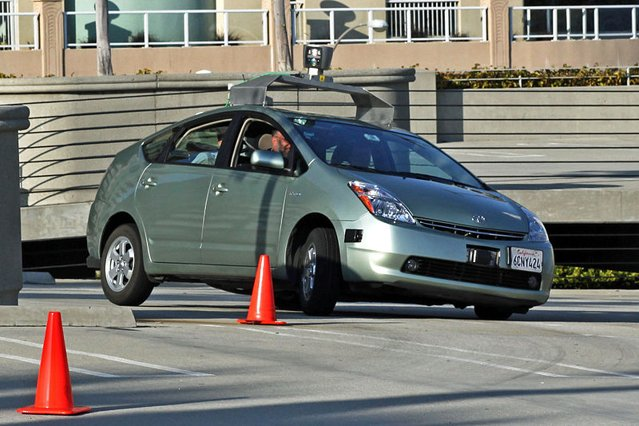
\includegraphics[width=1.0\linewidth]{images/GoogleCar.jpg}
        \caption{Google Car DriverLess}
      \end{figure}
    \end{minipage}
    &
    \begin{minipage}{0.5\linewidth}
      Velodyne LIDAR :
      \begin{itemize}
      \item 64 diodes laser
      \item 1.3 millions de points/secondes
      \item $360$\degre $\times~26.8$\degre
      \item Portée de 120 mètres
      \item Fragile
      \item 75.000\$
      \end{itemize}
      
      \begin{figure}
        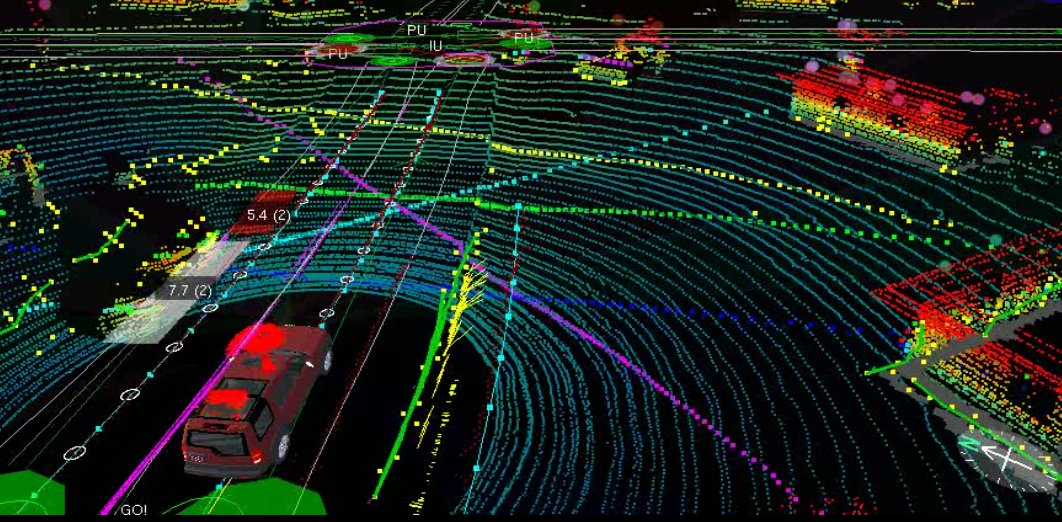
\includegraphics[width=0.8\linewidth]{images/LIDAR.jpg}
      \end{figure}
    \end{minipage}
  \end{tabular}
\end{frame}

\begin{frame}{Volvo}
  \begin{tabular}{c c}
    \begin{minipage}{0.5\linewidth}
      Convoi avec \textit{Leader} :
      \begin{itemize}
      \item Nécessite un véhicule de tête
      \item Sur route uniquement
      \item Nombreux capteurs
      \item Formation modifiable
      \item Haute vitesse (85 km/h)
      \end{itemize}
    \end{minipage}
    &
    \begin{minipage}{0.5\linewidth}
      \begin{figure}
        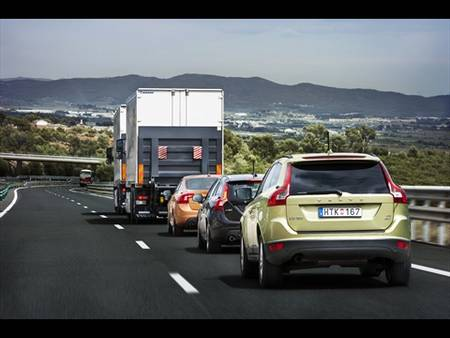
\includegraphics[width=1.0\linewidth]{images/ConvoiVolvo.jpg}
        \caption{Convoi de Volvo autonomes suivant un camion}
      \end{figure}
    \end{minipage}
  \end{tabular}
\end{frame}

\begin{frame}{Matériel}
  \begin{tabular}{c c}
    \begin{minipage}{0.5\linewidth}
      \begin{figure}
        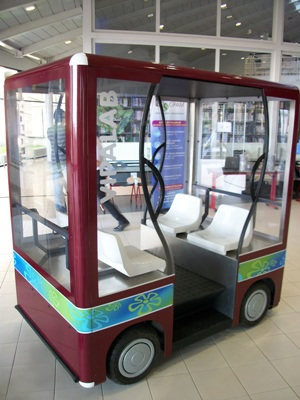
\includegraphics[width=0.8\linewidth]{images/VIPALAB.jpg}
        \caption{Un VipaLab produit par la société APOJEE}
      \end{figure}
    \end{minipage}
    &
    \begin{minipage}{0.5\linewidth}
      Caractéristiques :
      \begin{itemize}
      \item 100\% électrique
      \item 4 roues motrices
      \item 400 kg (hors batteries)
      \item 8 batteries 12V
      \item Vitesse maxi : 30km/h
      \item 3h d'autonomie
      \item Dimensions : $196\times127.3\times211$
      \end{itemize}
    \end{minipage}
  \end{tabular}
  %Guidage autonome réalisé par des capteurs de précision (doublage par des capteurs bas coût):
  %- GPS centimétrique (+ GPS bas coût).
  %- Caméras.
  %- Centrale inertielle (+ Gyromètre & Accéléromètre bas coûts).
  %- Odomètres sur roues (+ Odomètre sur variateur).
  %Sécurité assurée par trois niveaux de capteurs :
  %- Pare-choc sensitif.
  %- Capteurs ultrason.
  %- Radar à balayage laser.
  %
\end{frame}

\subsection*{Environnement}
\begin{frame}{Tests sur Pavin}

  \begin{figure}
    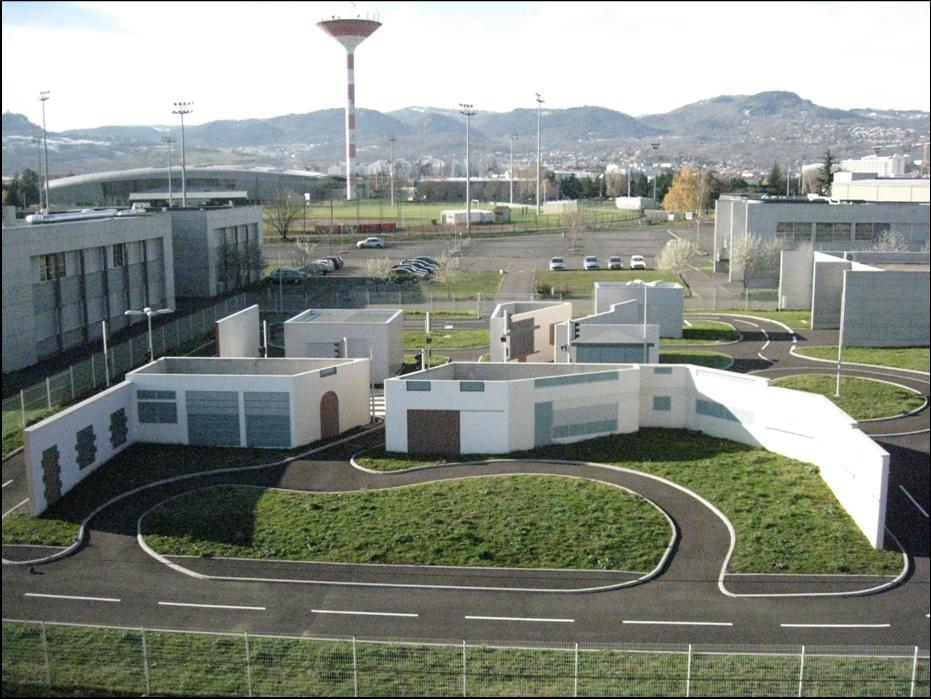
\includegraphics[width=0.7\linewidth]{images/pavin.jpg}
    \caption{Espace Pavin pour les simulations grandeur nature}
  \end{figure}
  % PAVIN is a site dedicated for intelligent urban vehicles. It is composed of 5000m2 space representing typical situation in urban environment: 317m of streets (asphalt) and 264m of open environment (sloppy ground, rough track). 
\end{frame}

%% --------------

\section{Recherche}
\subsection*{Recherche bibliographique}

\begin{frame}{Bibliographie}

  \begin{tabular}{c c}
    \begin{minipage}{0.4\linewidth}
      \begin{figure}
        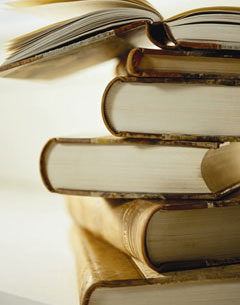
\includegraphics[width=0.6\linewidth]{images/bibliographie.jpg}
        \vspace{3mm}
        \onslide<2->{
        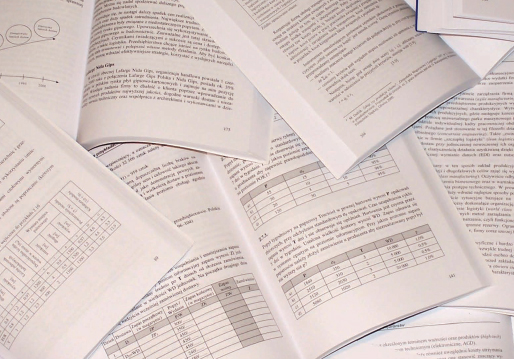
\includegraphics[width=0.9\linewidth]{images/publications.jpg}}
      \end{figure}
    \end{minipage}
    &
    \begin{minipage}{0.6\linewidth}
      \begin{itemize}
      \item Buts et objectifs
      \item Intérêts %Reconnaissance
        %\item Reconnaissance
      \item Inconvénients
        \vspace{5mm}
      \item<2-> Contenu actuel : %(121 ouvrages) :
        \begin{itemize}
        \item 3 livres
        \item 11 thèses
        \item 30 articles de journaux
        \item 74 conférences
        \item 3 autres
        \end{itemize}
      \end{itemize}
    \end{minipage}
  \end{tabular}
\end{frame}

\subsection*{Méthodes}

\begin{frame}{Recherche bibliographique}
  \begin{tabular}{c c}
    \begin{minipage}{0.6\linewidth}
      \begin{itemize}
      \item Où chercher ?
        \begin{itemize}
        \item Sites des Laboratoires
        \item Sites Personnels
        \item Conférences
        \item YouTube
        \item Google Scholar
        \end{itemize}
      \item<2-> Comment trouver ?
        \begin{itemize}
        \item Citations (publication / livre)
        \item Un nom
        \item Un robot
        \end{itemize}
      \item<3-> Disponibilité ?
        \begin{itemize}
        \item Site du laboratoire/université
        \item Site Personnel
        \item Achat
        \end{itemize}
        %\item Notions de maths dans les thèses
      \end{itemize}
    \end{minipage}
    &
    \begin{minipage}{0.4\linewidth}
      \begin{figure}
        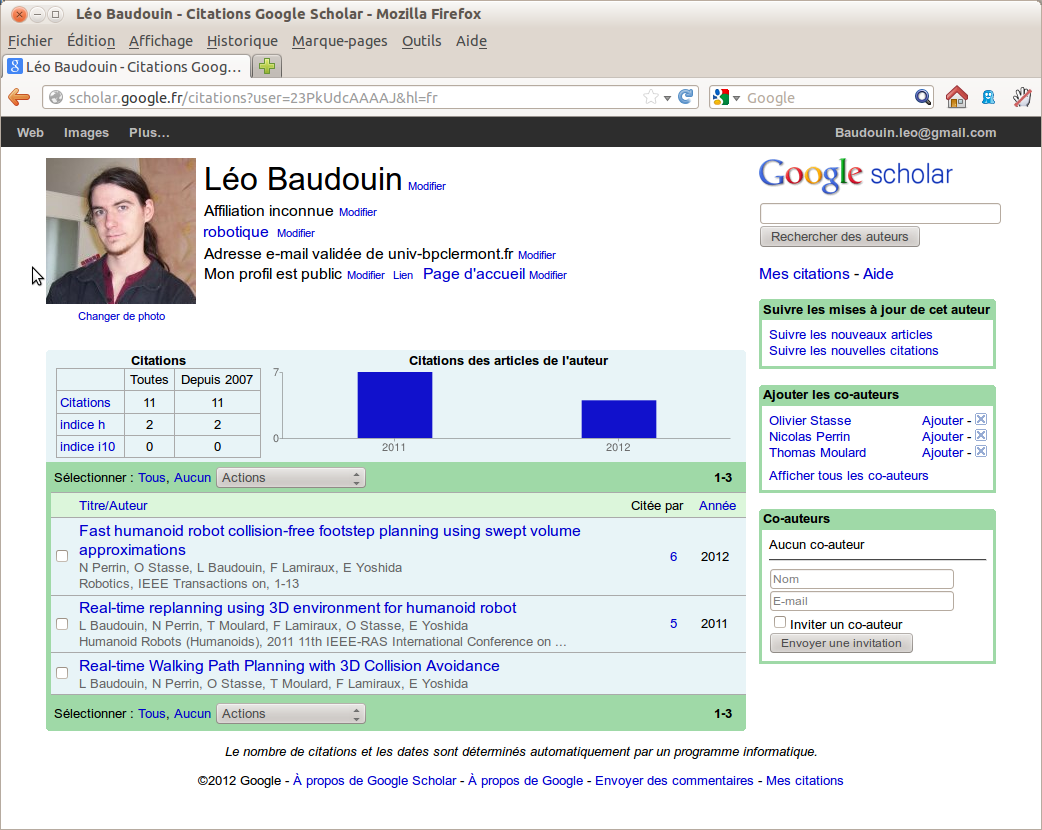
\includegraphics[width=0.9\linewidth]{images/GoogleScholar.png}
        \end{figure}
        \vspace{-3mm}
        \begin{figure}
        \onslide<2->{
        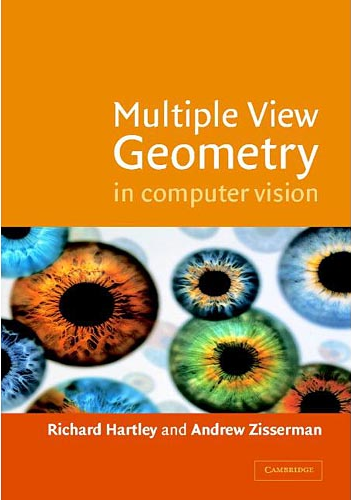
\includegraphics[width=0.5\linewidth]{images/Book.png}}
      \end{figure}
    \end{minipage}
  \end{tabular}
\end{frame}


\subsection*{Gestion Bibliographique}

\begin{frame}
  \begin{figure}
    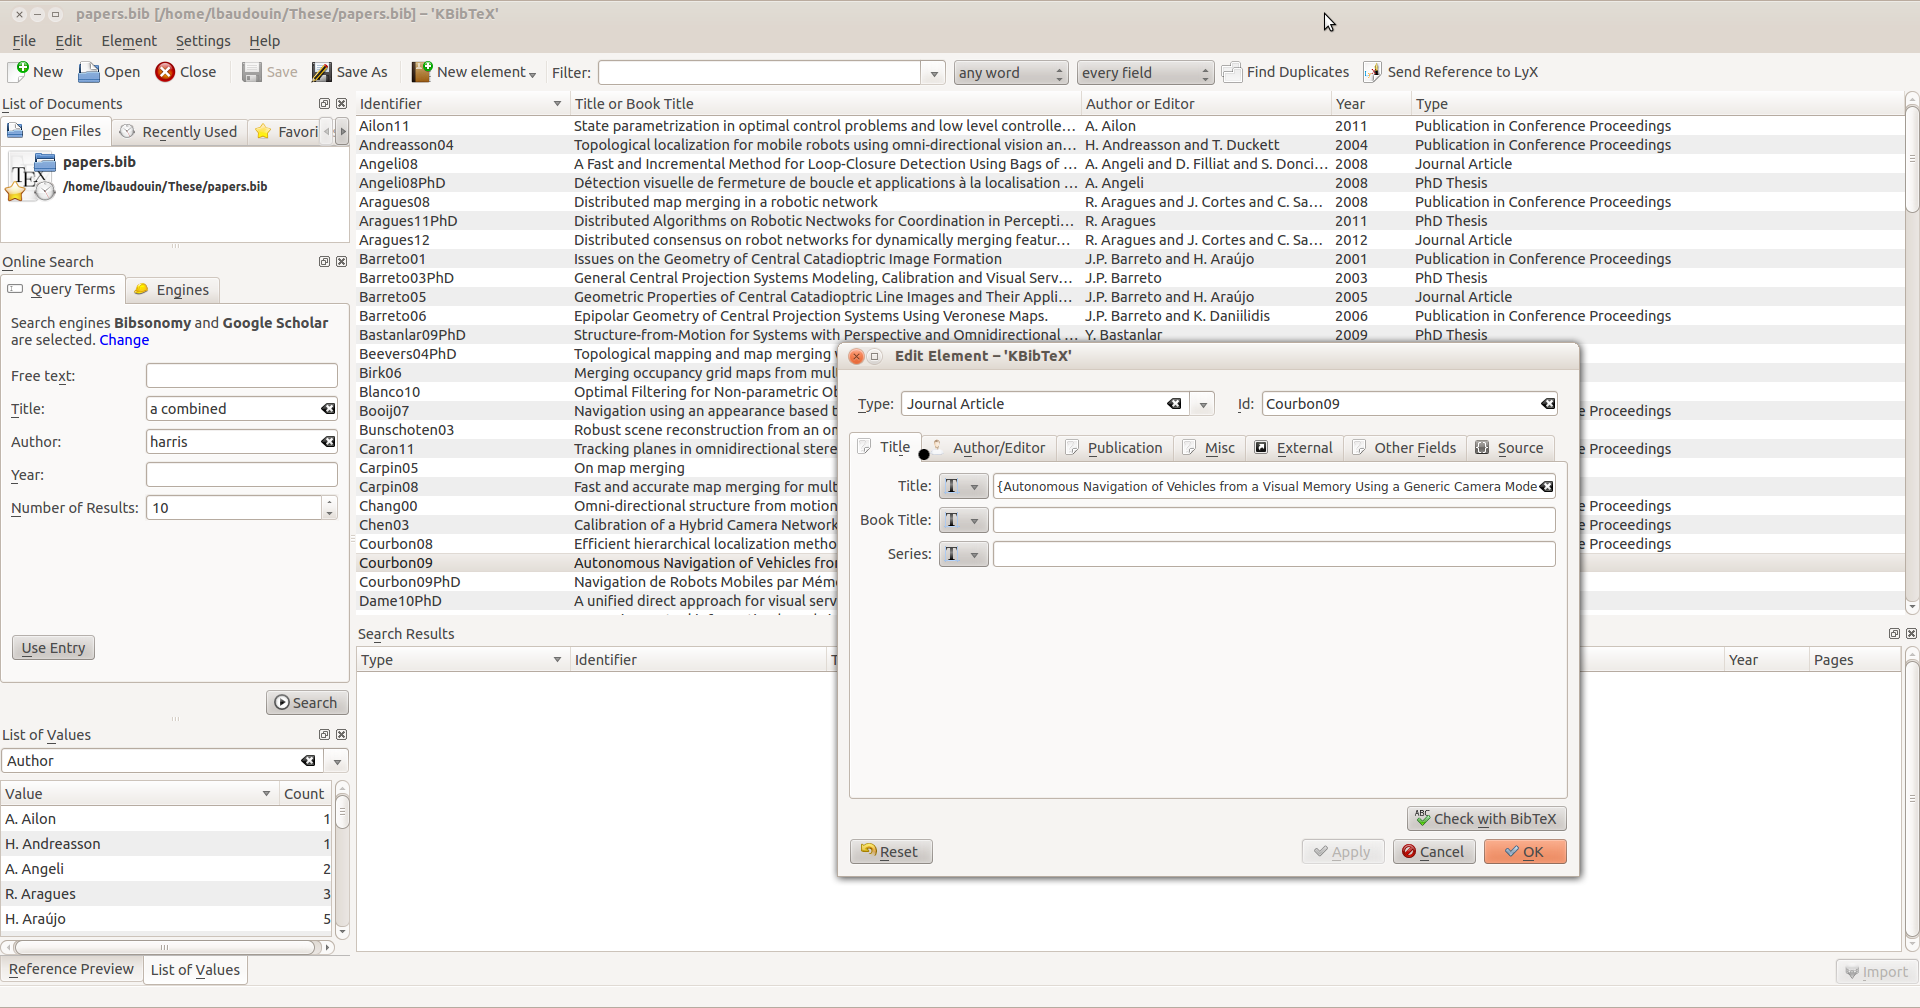
\includegraphics[width=1.0\linewidth]{images/KBibTex.png}
    \caption{Capture d'écran de KBibTex, logiciel libre de gestion de bibliographie avec recherche intégrée}
  \end{figure}
\end{frame}

\subsection*{Articles}

\begin{frame}{Exemple}
  %Auteurs, écriture, publication (tro, iros, \dots)

  Exemple :\\
  \vspace{2mm}
  %\begin{tiny}
  \begin{scriptsize}
    @inproceedings$\lbrace$ baudouin\string:humanoids\string:11,\\
    \hspace{5mm} author = "L. Baudouin and N. Perrin and T. Moulard and F. Lamiraux and\\
    \hspace{19mm} O. Stasse and E. Yoshida",\\
    \hspace{5mm} booktitle = "\{IEEE/RAS International Conference on Humanoid Robotics\\
    \hspace{22mm} (Humanoids'11)\}",\\
    \hspace{5mm} title = "\{Real-time Replanning Using 3D Environment for Humanoid Robot\}",\\
    \hspace{5mm} url = "http://ubuntuone.com/6zyz487WVECpyW88tEfQz5",\\
    \hspace{5mm} year = "2011"\\
    \vspace{-2mm}
    $\rbrace$
  \end{scriptsize}
  %\end{tiny}
  \vspace{5mm}

  Article :\\
  \begin{scriptsize}
    \mbox{
      \citeauthor{baudouin:humanoids:11}
      \citetitle{baudouin:humanoids:11}
      \cite{baudouin:humanoids:11}
    }
  \end{scriptsize}
  %\vspace{5mm}

  Thèse :\\
  \begin{scriptsize}
    \mbox{
      \citeauthor{Courbon09PhD}
      \citetitle{Courbon09PhD}
      \cite{Courbon09PhD}}
  \end{scriptsize}
  \vspace{5mm}

\end{frame}

\begin{frame}{Exemple}
  %\begin{minipage}{0.5\linewidth}
  \printbibliography[heading=none]
  %\end{minipage}
\end{frame}

%% --------------

\section{Avancement}

\subsection*{Vision}
\begin{frame}{Reconstruction 3D}
  \begin{tabular}{c c}
    \begin{minipage}{0.5\linewidth}
      \begin{figure}
        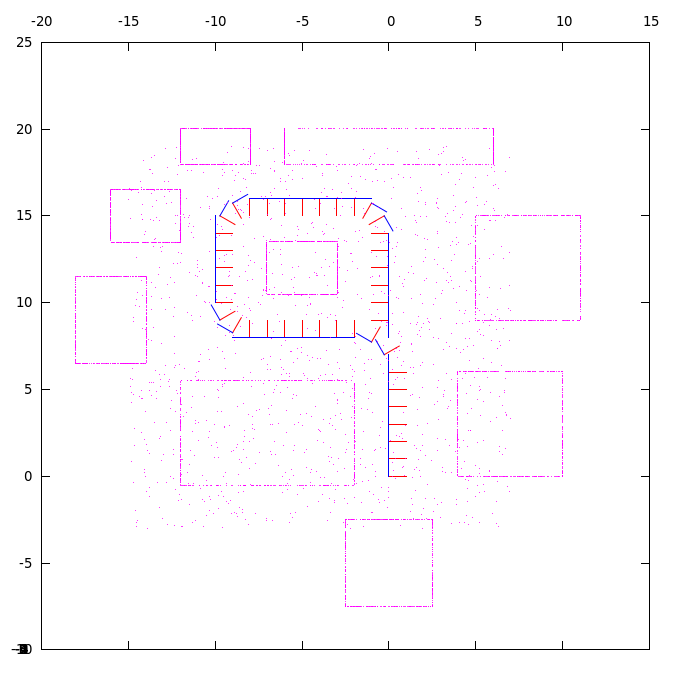
\includegraphics[width=0.9\linewidth]{images/createimages.png}
        \caption{Simulation d'un environnement}
      \end{figure}
    \end{minipage}
    &
    \begin{minipage}{0.5\linewidth}
      \begin{figure}
        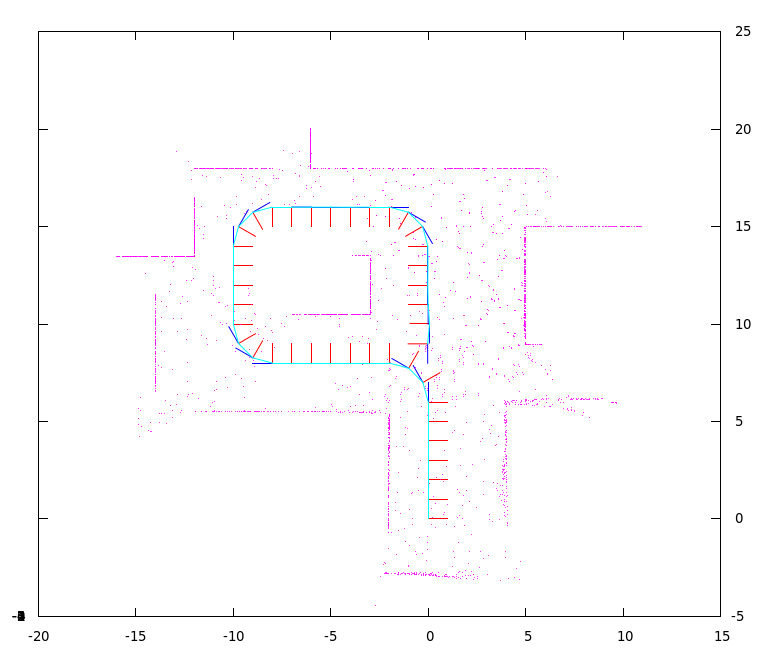
\includegraphics[width=1.0\linewidth]{images/buildfromvideo.png}
        \caption{Reconstruction à partir des points 2D}
      \end{figure}
    \end{minipage}
  \end{tabular}
\end{frame}

\begin{frame}{Images Réelles}
  \begin{figure}
    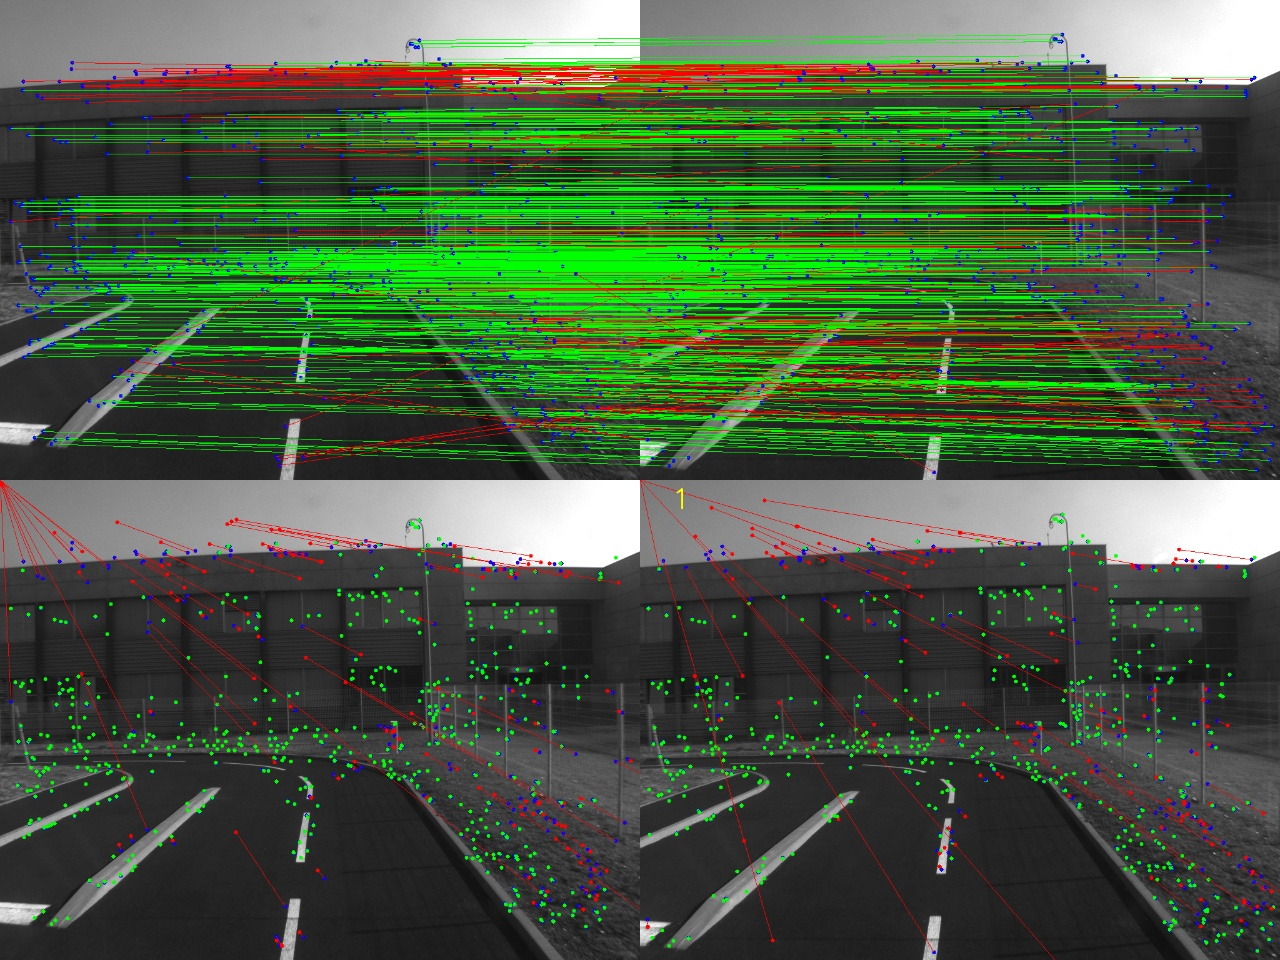
\includegraphics[width=0.7\linewidth]{images/result.jpg}
    \caption{Résultat des appariements de points}
  \end{figure}
\end{frame}


\subsection*{Navigation}
\begin{frame}{Formation}
  \begin{center}
    \begin{Large}
      \textbf{Cahier des charges}
    \end{Large}
  \end{center}
  \begin{tabular}{c c}
    \begin{minipage}{0.6\linewidth}
      \begin{description}
      \item[Application] Déplacement en convoi
      \item[Formation] En ligne
      \item[Nombre] 2 à 6 véhicules
      \item[Distance] Entre 50cm et 2m
      \item[Leader] Avec
      \item[Modularité] Entrer/Sortir du convoi
      \item[Projets] Semblable à celui de Volvo
      \end{description}
    \end{minipage}
    &
    \begin{minipage}{0.4\linewidth}
      \begin{figure}
        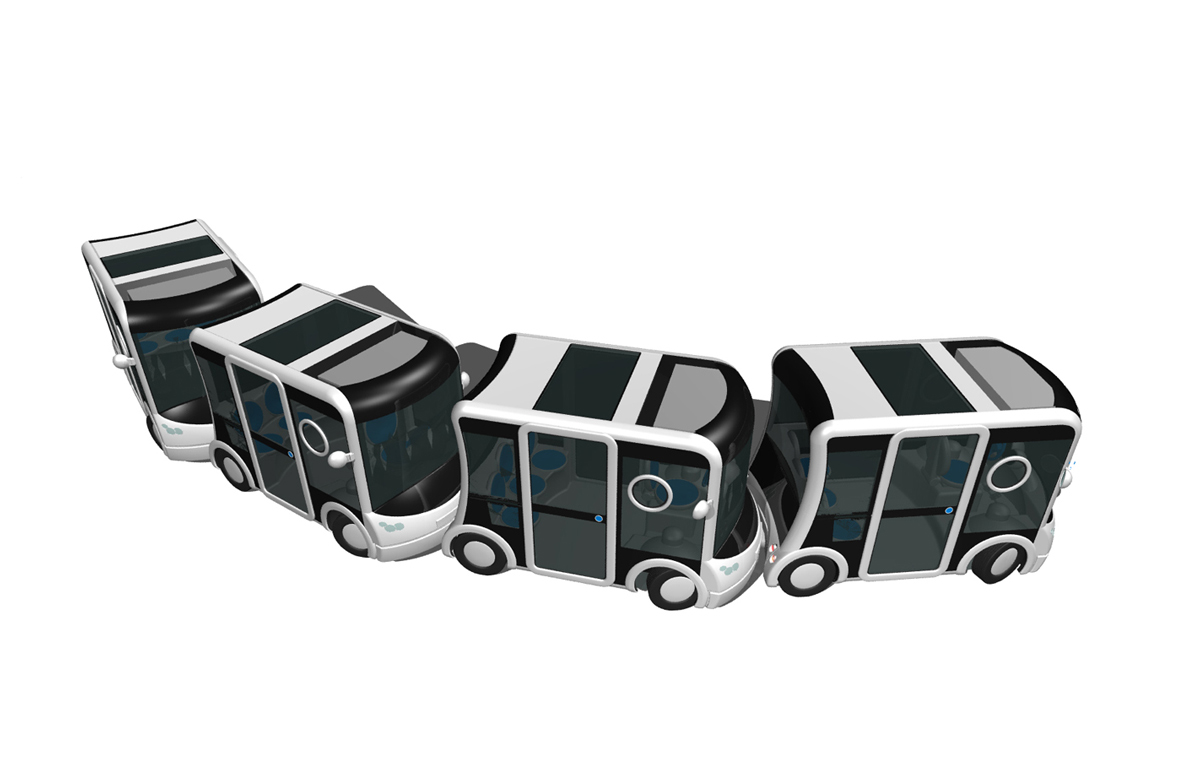
\includegraphics[width=1.0\linewidth]{images/convoi.jpg}
        \caption{Véhicules autonomes en convoi/formation}
      \end{figure}
    \end{minipage}
  \end{tabular}

\end{frame}

\subsection*{Tests Réalisés}
\begin{frame}{Développement}
  \begin{center}
    \begin{Large}
      \textbf{Programmes et librairies testés}
    \end{Large}
  \end{center}
  \begin{itemize}
  \item Sovin (SOftware for VIsual Navigation)
  \item loop\_closure
  \item SSBA (Simple Sparse Bundle Adjustment)
  \item RobotVision
  \item ScaViSLAM
  \item ICP (Iterative Closest Point)
  \item MRPT (Mobile Robot Programming Toolkit)
  \end{itemize}
\end{frame}

\subsection*{Situation actuelle}
\begin{frame}{Problèmes rencontrés}

  \begin{tabular}{c | c}
    \begin{minipage}{0.5\linewidth}
      \begin{center}
        \begin{Large}
          \textbf{Programmes}
        \end{Large}
      \end{center}
      \begin{itemize}
      \item Notions mathématiques
      \item Disponibilité des programmes
      \item C++ vs Matlab
      \item Jeu d'images calibré
      \end{itemize}
    \end{minipage}
    &
        \onslide<2->{
    \begin{minipage}{0.5\linewidth}
      \begin{center}
        \begin{Large}
          \textbf{Thèse}
        \end{Large}
      \end{center}
      \begin{itemize}
      \item Nombre important de publications
      \item Objectifs parfois flous
      \item Retard cumulé
      \item Confiance en soi
      \end{itemize}
    \end{minipage}}
  \end{tabular}
\end{frame}

%% --------------

\section{Conclusion}
\subsection*{Objectifs}
\begin{frame}{Suite des travaux}
  \begin{tabular}{c c}
    \begin{minipage}{0.5\linewidth}
      A mettre en place en deux ans :
      \begin{enumerate}
      \item Navigation Classique
      \item Navigation Topologique %Graphe : Noeuds + distance (arc)
      \item Mise en Formation
      \item Déplacements en Formation
      \item Surveillance \& Suivi de Cible
      \end{enumerate}
    \end{minipage}
    &
    \begin{minipage}{0.5\linewidth}
      \begin{figure}
        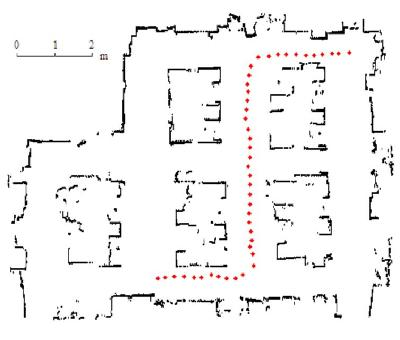
\includegraphics[width=0.8\linewidth]{images/navigation.jpg}\\
        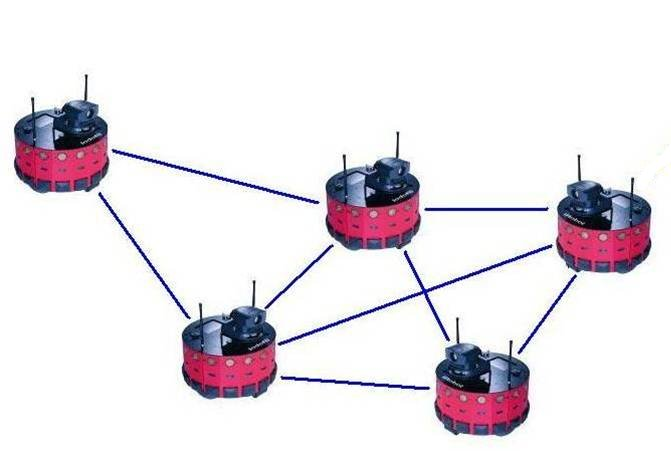
\includegraphics[width=0.8\linewidth]{images/formation.jpg}
      \end{figure}
    \end{minipage}
  \end{tabular}

\end{frame}

\subsection*{Six mois de Stage}
\begin{frame}{Conclusion}
  \begin{figure}
    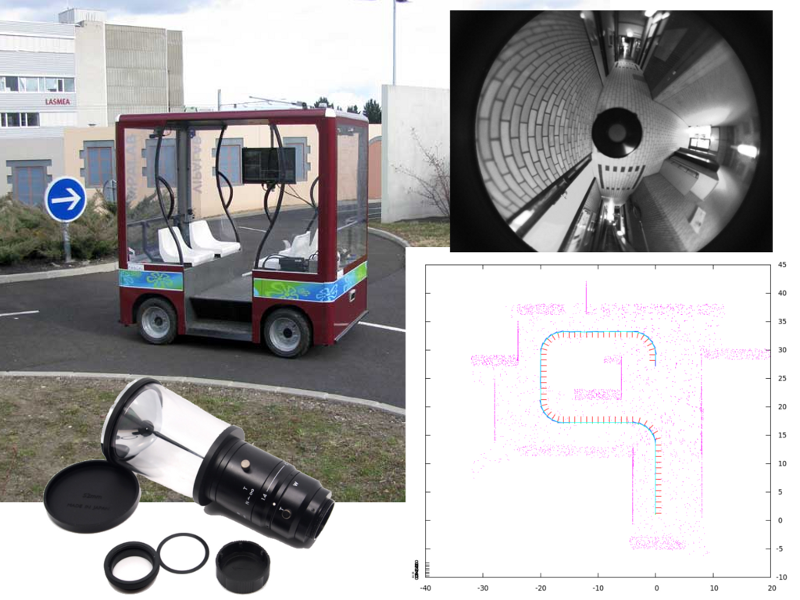
\includegraphics[width=0.7\linewidth]{images/conclusion.png}
  \end{figure}
\end{frame}


\end{document}  
